% IEEE conference format.  On Overleaf (IEEEtran.cls available) this compiles
% as an IEEE conference paper; elsewhere a close stand-in (ieee-fallback.sty)
% is used.  Every number comes from numbers.tex (python report/make_numbers.py).
\IfFileExists{IEEEtran.cls}{%
  \documentclass[conference]{IEEEtran}}{%
  \documentclass[10pt,twocolumn,letterpaper]{article}\usepackage{ieee-fallback}}
\usepackage[utf8]{inputenc}
\usepackage[T1]{fontenc}
\usepackage{amsmath,amssymb}
\usepackage{graphicx}
\usepackage{booktabs}
\usepackage{xcolor}
\usepackage[hidelinks]{hyperref}
\usepackage{cite}
\usepackage{placeins}
% generated by report/make_numbers.py from results/*.csv -- do not edit
\newcommand{\AgentAppliedAll}{16}
\newcommand{\AgentAppliedTemplate}{15}
\newcommand{\AgentAppliedTotal}{6}
\newcommand{\AgentCallLatMed}{2.27}
\newcommand{\AgentCallsHour}{7.65}
\newcommand{\AgentChanges}{6}
\newcommand{\AgentDecHour}{3.83}
\newcommand{\AgentDecisions}{287}
\newcommand{\AgentHost}{x86_64 2 CPU threads}
\newcommand{\AgentInvalid}{46}
\newcommand{\AgentLatMed}{5.78}
\newcommand{\AgentLatPninetyfive}{14.67}
\newcommand{\AgentModel}{qwen3-0.6b-q4km}
\newcommand{\AgentRbw}{0}
\newcommand{\AgentRuns}{25}
\newcommand{\AgentSetCalls}{11}
\newcommand{\AgentSetRejected}{5}
\newcommand{\AgentToolsPerDec}{1.22}
\newcommand{\AlohaMaxErr}{0.0026}
\newcommand{\AlohaMaxG}{1.03}
\newcommand{\AppliedNoFacts}{0}
\newcommand{\AppliedNoTool}{0}
\newcommand{\CritASFeleven}{150.0}
\newcommand{\CritASFnine}{800.0}
\newcommand{\CritASFten}{200.0}
\newcommand{\CritASFtwelve}{50.0}
\newcommand{\CritBSFeleven}{$>$1000}
\newcommand{\CritBSFnine}{$>$1000}
\newcommand{\CritBSFten}{$>$1000}
\newcommand{\CritBSFtwelve}{300.0}
\newcommand{\DecisionsNoFacts}{271}
\newcommand{\DecisionsNoTool}{271}
\newcommand{\DetPrecision}{0.92}
\newcommand{\DetRecall}{1.00}
\newcommand{\DriftBinsSFtwelve}{9.23}
\newcommand{\EoneGapMax}{0.32}
\newcommand{\EoneGapMin}{-1.40}
\newcommand{\EoneGapSFtwelve}{-1.4}
\newcommand{\EoneMCMaxDiff}{0.020}
\newcommand{\EoneMCTrials}{2000}
\newcommand{\EthreeAgentEqualUpTo}{200}
\newcommand{\EthreeAgentLossRuns}{7}
\newcommand{\EthreeAgentRuns}{30}
\newcommand{\EthreeAgentWorst}{$-$15.5}
\newcommand{\EthreeAgentWorstN}{800}
\newcommand{\EthreeEADRHi}{15.7}
\newcommand{\EthreeEADRLo}{16.1}
\newcommand{\EthreeEAgentHi}{20.6}
\newcommand{\EthreeEAgentLo}{16.1}
\newcommand{\EthreeEMLHi}{9.3}
\newcommand{\EthreeEMLLo}{9.9}
\newcommand{\EthreeEOracleHi}{9.2}
\newcommand{\EthreeEOracleLo}{9.1}
\newcommand{\EthreeERulesHi}{15.7}
\newcommand{\EthreeERulesLo}{16.1}
\newcommand{\EthreeESFsevenHi}{6.7}
\newcommand{\EthreeESFsevenLo}{6.6}
\newcommand{\EthreeESFtwelveHi}{317.0}
\newcommand{\EthreeESFtwelveLo}{146.8}
\newcommand{\EthreeNhi}{1000}
\newcommand{\EthreeNlo}{100}
\newcommand{\EthreePdrADRHi}{95.4}
\newcommand{\EthreePdrADRLo}{97.5}
\newcommand{\EthreePdrAgentHi}{93.3}
\newcommand{\EthreePdrAgentLo}{97.5}
\newcommand{\EthreePdrMLHi}{75.4}
\newcommand{\EthreePdrMLLo}{76.3}
\newcommand{\EthreePdrOracleHi}{89.4}
\newcommand{\EthreePdrOracleLo}{98.1}
\newcommand{\EthreePdrRulesHi}{95.4}
\newcommand{\EthreePdrRulesLo}{97.5}
\newcommand{\EthreePdrSFsevenHi}{84.8}
\newcommand{\EthreePdrSFsevenLo}{86.7}
\newcommand{\EthreePdrSFtwelveHi}{41.9}
\newcommand{\EthreePdrSFtwelveLo}{90.4}
\newcommand{\EthreePdrSdADRHi}{0.2}
\newcommand{\EthreePdrSdADRLo}{0.6}
\newcommand{\EthreePdrSdAgentHi}{4.6}
\newcommand{\EthreePdrSdAgentLo}{0.6}
\newcommand{\EthreePdrSdMLHi}{0.3}
\newcommand{\EthreePdrSdMLLo}{1.6}
\newcommand{\EthreePdrSdOracleHi}{0.2}
\newcommand{\EthreePdrSdOracleLo}{0.3}
\newcommand{\EthreePdrSdRulesHi}{0.2}
\newcommand{\EthreePdrSdRulesLo}{0.7}
\newcommand{\EthreePdrSdSFsevenHi}{0.8}
\newcommand{\EthreePdrSdSFsevenLo}{3.0}
\newcommand{\EthreePdrSdSFtwelveHi}{0.6}
\newcommand{\EthreePdrSdSFtwelveLo}{1.3}
\newcommand{\EtwoAshareSFtwelve}{39}
\newcommand{\EtwoAshareSFtwelveSnr}{100}
\newcommand{\EtwoBSFtwelveZenithFrom}{650}
\newcommand{\EtwoBshareSFtwelve}{98}
\newcommand{\EtwoDelayMax}{6.4}
\newcommand{\EtwoDelayMin}{2.0}
\newcommand{\EtwoDuration}{8.5}
\newcommand{\EtwoMaxDoppler}{19.7}
\newcommand{\EtwoMaxRate}{252}
\newcommand{\EtwoRateFiveFifty}{279.2}
\newcommand{\EtwoSnrMax}{-9.8}
\newcommand{\EtwoSnrMin}{-19.9}
\newcommand{\OkASFeleven}{100}
\newcommand{\OkASFnine}{600}
\newcommand{\OkASFten}{150}
\newcommand{\OkASFtwelve}{25}
\newcommand{\OkBSFeleven}{1000}
\newcommand{\OkBSFnine}{1000}
\newcommand{\OkBSFten}{1000}
\newcommand{\OkBSFtwelve}{250}
\newcommand{\PerPackets}{400}
\newcommand{\SFiveAgentRunsActed}{2}
\newcommand{\SFiveCensADR}{0}
\newcommand{\SFiveCensAgent}{0}
\newcommand{\SFiveCensML}{0}
\newcommand{\SFiveCensOracle}{0}
\newcommand{\SFiveCensRules}{0}
\newcommand{\SFiveCensSFseven}{0}
\newcommand{\SFiveCensSFtwelve}{0}
\newcommand{\SFiveDetDelay}{6}
\newcommand{\SFiveDetPrec}{0.87}
\newcommand{\SFiveDiffAgent}{$-$17.5}
\newcommand{\SFiveDiffML}{$-$20.1}
\newcommand{\SFiveDiffOracle}{$-$7.8}
\newcommand{\SFiveDiffRules}{+0.5}
\newcommand{\SFiveDiffSFseven}{$-$11.3}
\newcommand{\SFiveDiffSFtwelve}{$-$50.8}
\newcommand{\SFiveDiffSdAgent}{23.9}
\newcommand{\SFiveDiffSdML}{1.1}
\newcommand{\SFiveDiffSdOracle}{0.4}
\newcommand{\SFiveDiffSdRules}{0.2}
\newcommand{\SFiveDiffSdSFseven}{2.0}
\newcommand{\SFiveDiffSdSFtwelve}{1.2}
\newcommand{\SFiveEADR}{14.4}
\newcommand{\SFiveEAgent}{82.1}
\newcommand{\SFiveEML}{8.0}
\newcommand{\SFiveEOracle}{9.2}
\newcommand{\SFiveERules}{15.0}
\newcommand{\SFiveESFseven}{6.9}
\newcommand{\SFiveESFtwelve}{306.9}
\newcommand{\SFiveLossesAgent}{2}
\newcommand{\SFiveLossesML}{5}
\newcommand{\SFiveLossesOracle}{5}
\newcommand{\SFiveLossesRules}{0}
\newcommand{\SFiveLossesSFseven}{5}
\newcommand{\SFiveLossesSFtwelve}{5}
\newcommand{\SFivePdrADR}{94.1}
\newcommand{\SFivePdrAgent}{76.6}
\newcommand{\SFivePdrML}{74.0}
\newcommand{\SFivePdrNoFacts}{94.1}
\newcommand{\SFivePdrNoTool}{94.1}
\newcommand{\SFivePdrOracle}{86.3}
\newcommand{\SFivePdrRules}{94.6}
\newcommand{\SFivePdrSFseven}{82.8}
\newcommand{\SFivePdrSFtwelve}{43.3}
\newcommand{\SFivePdrSdADR}{0.4}
\newcommand{\SFivePdrSdAgent}{23.9}
\newcommand{\SFivePdrSdML}{0.8}
\newcommand{\SFivePdrSdNoFacts}{0.4}
\newcommand{\SFivePdrSdNoTool}{0.4}
\newcommand{\SFivePdrSdOracle}{0.5}
\newcommand{\SFivePdrSdRules}{0.4}
\newcommand{\SFivePdrSdSFseven}{1.9}
\newcommand{\SFivePdrSdSFtwelve}{0.9}
\newcommand{\SFiveRdrADR}{94.6}
\newcommand{\SFiveRdrAgent}{83.2}
\newcommand{\SFiveRdrML}{75.6}
\newcommand{\SFiveRdrOracle}{90.4}
\newcommand{\SFiveRdrRules}{94.8}
\newcommand{\SFiveRdrSFseven}{84.5}
\newcommand{\SFiveRdrSFtwelve}{52.5}
\newcommand{\SFiveRecADR}{2}
\newcommand{\SFiveRecAgent}{18}
\newcommand{\SFiveRecML}{2}
\newcommand{\SFiveRecOracle}{30}
\newcommand{\SFiveRecRules}{2}
\newcommand{\SFiveRecSFseven}{8}
\newcommand{\SFiveRecSFtwelve}{56}
\newcommand{\SFiveWinsAgent}{0}
\newcommand{\SFiveWinsML}{0}
\newcommand{\SFiveWinsOracle}{0}
\newcommand{\SFiveWinsRules}{5}
\newcommand{\SFiveWinsSFseven}{0}
\newcommand{\SFiveWinsSFtwelve}{0}
\newcommand{\SFourAgentRunsActed}{2}
\newcommand{\SFourCensADR}{0}
\newcommand{\SFourCensAgent}{1}
\newcommand{\SFourCensML}{0}
\newcommand{\SFourCensOracle}{0}
\newcommand{\SFourCensRules}{0}
\newcommand{\SFourCensSFseven}{0}
\newcommand{\SFourCensSFtwelve}{0}
\newcommand{\SFourDetDelay}{5}
\newcommand{\SFourDetPrec}{0.92}
\newcommand{\SFourDiffAgent}{$-$0.1}
\newcommand{\SFourDiffML}{$-$5.1}
\newcommand{\SFourDiffOracle}{+62.3}
\newcommand{\SFourDiffRules}{+12.9}
\newcommand{\SFourDiffSFseven}{$-$5.6}
\newcommand{\SFourDiffSFtwelve}{$-$4.3}
\newcommand{\SFourDiffSdAgent}{0.1}
\newcommand{\SFourDiffSdML}{0.7}
\newcommand{\SFourDiffSdOracle}{1.7}
\newcommand{\SFourDiffSdRules}{0.5}
\newcommand{\SFourDiffSdSFseven}{0.5}
\newcommand{\SFourDiffSdSFtwelve}{0.5}
\newcommand{\SFourEADR}{156.8}
\newcommand{\SFourEAgent}{157.2}
\newcommand{\SFourEML}{143.3}
\newcommand{\SFourEOracle}{43.7}
\newcommand{\SFourERules}{89.2}
\newcommand{\SFourESFseven}{31.7}
\newcommand{\SFourESFtwelve}{690.5}
\newcommand{\SFourLossesAgent}{1}
\newcommand{\SFourLossesML}{5}
\newcommand{\SFourLossesOracle}{0}
\newcommand{\SFourLossesRules}{0}
\newcommand{\SFourLossesSFseven}{5}
\newcommand{\SFourLossesSFtwelve}{5}
\newcommand{\SFourPdrADR}{23.5}
\newcommand{\SFourPdrAgent}{23.5}
\newcommand{\SFourPdrML}{18.4}
\newcommand{\SFourPdrNoFacts}{23.5}
\newcommand{\SFourPdrNoTool}{23.5}
\newcommand{\SFourPdrOracle}{85.8}
\newcommand{\SFourPdrRules}{36.5}
\newcommand{\SFourPdrSFseven}{18.0}
\newcommand{\SFourPdrSFtwelve}{19.2}
\newcommand{\SFourPdrSdADR}{0.3}
\newcommand{\SFourPdrSdAgent}{0.4}
\newcommand{\SFourPdrSdML}{0.8}
\newcommand{\SFourPdrSdNoFacts}{0.3}
\newcommand{\SFourPdrSdNoTool}{0.3}
\newcommand{\SFourPdrSdOracle}{1.5}
\newcommand{\SFourPdrSdRules}{0.6}
\newcommand{\SFourPdrSdSFseven}{0.6}
\newcommand{\SFourPdrSdSFtwelve}{0.5}
\newcommand{\SFourRdrADR}{69.3}
\newcommand{\SFourRdrAgent}{67.3}
\newcommand{\SFourRdrML}{55.9}
\newcommand{\SFourRdrOracle}{76.0}
\newcommand{\SFourRdrRules}{71.5}
\newcommand{\SFourRdrSFseven}{58.6}
\newcommand{\SFourRdrSFtwelve}{56.1}
\newcommand{\SFourRecADR}{30}
\newcommand{\SFourRecAgent}{30}
\newcommand{\SFourRecML}{30}
\newcommand{\SFourRecOracle}{26}
\newcommand{\SFourRecRules}{30}
\newcommand{\SFourRecSFseven}{44}
\newcommand{\SFourRecSFtwelve}{50}
\newcommand{\SFourWinsAgent}{0}
\newcommand{\SFourWinsML}{0}
\newcommand{\SFourWinsOracle}{5}
\newcommand{\SFourWinsRules}{5}
\newcommand{\SFourWinsSFseven}{0}
\newcommand{\SFourWinsSFtwelve}{0}
\newcommand{\SOneAgentRunsActed}{0}
\newcommand{\SOneCensADR}{0}
\newcommand{\SOneCensAgent}{0}
\newcommand{\SOneCensML}{0}
\newcommand{\SOneCensOracle}{0}
\newcommand{\SOneCensRules}{0}
\newcommand{\SOneCensSFseven}{0}
\newcommand{\SOneCensSFtwelve}{0}
\newcommand{\SOneDetDelay}{1}
\newcommand{\SOneDetPrec}{0.95}
\newcommand{\SOneDiffAgent}{+0.0}
\newcommand{\SOneDiffML}{$-$16.6}
\newcommand{\SOneDiffOracle}{+21.4}
\newcommand{\SOneDiffRules}{+10.5}
\newcommand{\SOneDiffSFseven}{$-$1.8}
\newcommand{\SOneDiffSFtwelve}{$-$2.8}
\newcommand{\SOneDiffSdAgent}{0.0}
\newcommand{\SOneDiffSdML}{1.7}
\newcommand{\SOneDiffSdOracle}{0.9}
\newcommand{\SOneDiffSdRules}{1.2}
\newcommand{\SOneDiffSdSFseven}{1.8}
\newcommand{\SOneDiffSdSFtwelve}{0.9}
\newcommand{\SOneEADR}{20.5}
\newcommand{\SOneEAgent}{20.5}
\newcommand{\SOneEML}{10.6}
\newcommand{\SOneEOracle}{8.7}
\newcommand{\SOneERules}{18.3}
\newcommand{\SOneESFseven}{7.8}
\newcommand{\SOneESFtwelve}{183.8}
\newcommand{\SOneLossesAgent}{0}
\newcommand{\SOneLossesML}{5}
\newcommand{\SOneLossesOracle}{0}
\newcommand{\SOneLossesRules}{0}
\newcommand{\SOneLossesSFseven}{5}
\newcommand{\SOneLossesSFtwelve}{5}
\newcommand{\SOnePdrADR}{75.1}
\newcommand{\SOnePdrAgent}{75.1}
\newcommand{\SOnePdrML}{58.4}
\newcommand{\SOnePdrNoFacts}{75.1}
\newcommand{\SOnePdrNoTool}{75.1}
\newcommand{\SOnePdrOracle}{96.5}
\newcommand{\SOnePdrRules}{85.6}
\newcommand{\SOnePdrSFseven}{73.3}
\newcommand{\SOnePdrSFtwelve}{72.3}
\newcommand{\SOnePdrSdADR}{0.8}
\newcommand{\SOnePdrSdAgent}{0.8}
\newcommand{\SOnePdrSdML}{1.4}
\newcommand{\SOnePdrSdNoFacts}{0.8}
\newcommand{\SOnePdrSdNoTool}{0.8}
\newcommand{\SOnePdrSdOracle}{0.8}
\newcommand{\SOnePdrSdRules}{1.8}
\newcommand{\SOnePdrSdSFseven}{1.3}
\newcommand{\SOnePdrSdSFtwelve}{1.3}
\newcommand{\SOneRdrADR}{92.3}
\newcommand{\SOneRdrAgent}{92.3}
\newcommand{\SOneRdrML}{73.9}
\newcommand{\SOneRdrOracle}{96.1}
\newcommand{\SOneRdrRules}{94.6}
\newcommand{\SOneRdrSFseven}{83.6}
\newcommand{\SOneRdrSFtwelve}{74.9}
\newcommand{\SOneRecADR}{30}
\newcommand{\SOneRecAgent}{30}
\newcommand{\SOneRecML}{30}
\newcommand{\SOneRecOracle}{0}
\newcommand{\SOneRecRules}{24}
\newcommand{\SOneRecSFseven}{38}
\newcommand{\SOneRecSFtwelve}{44}
\newcommand{\SOneWinsAgent}{0}
\newcommand{\SOneWinsML}{0}
\newcommand{\SOneWinsOracle}{5}
\newcommand{\SOneWinsRules}{5}
\newcommand{\SOneWinsSFseven}{0}
\newcommand{\SOneWinsSFtwelve}{0}
\newcommand{\SThreeAgentRunsActed}{0}
\newcommand{\SThreeCensADR}{3}
\newcommand{\SThreeCensAgent}{3}
\newcommand{\SThreeCensML}{2}
\newcommand{\SThreeCensOracle}{0}
\newcommand{\SThreeCensRules}{0}
\newcommand{\SThreeCensSFseven}{1}
\newcommand{\SThreeCensSFtwelve}{4}
\newcommand{\SThreeDiffAgent}{+0.0}
\newcommand{\SThreeDiffML}{$-$19.9}
\newcommand{\SThreeDiffOracle}{+13.0}
\newcommand{\SThreeDiffRules}{+15.0}
\newcommand{\SThreeDiffSFseven}{$-$12.1}
\newcommand{\SThreeDiffSFtwelve}{$-$15.4}
\newcommand{\SThreeDiffSdAgent}{0.0}
\newcommand{\SThreeDiffSdML}{1.8}
\newcommand{\SThreeDiffSdOracle}{1.4}
\newcommand{\SThreeDiffSdRules}{1.2}
\newcommand{\SThreeDiffSdSFseven}{0.7}
\newcommand{\SThreeDiffSdSFtwelve}{0.7}
\newcommand{\SThreeEADR}{45.0}
\newcommand{\SThreeEAgent}{45.0}
\newcommand{\SThreeEML}{42.1}
\newcommand{\SThreeEOracle}{20.3}
\newcommand{\SThreeERules}{19.9}
\newcommand{\SThreeESFseven}{8.1}
\newcommand{\SThreeESFtwelve}{199.3}
\newcommand{\SThreeLossesAgent}{0}
\newcommand{\SThreeLossesML}{5}
\newcommand{\SThreeLossesOracle}{0}
\newcommand{\SThreeLossesRules}{0}
\newcommand{\SThreeLossesSFseven}{5}
\newcommand{\SThreeLossesSFtwelve}{5}
\newcommand{\SThreePdrADR}{82.0}
\newcommand{\SThreePdrAgent}{82.0}
\newcommand{\SThreePdrML}{62.1}
\newcommand{\SThreePdrNoFacts}{82.0}
\newcommand{\SThreePdrNoTool}{82.0}
\newcommand{\SThreePdrOracle}{95.1}
\newcommand{\SThreePdrRules}{97.1}
\newcommand{\SThreePdrSFseven}{69.9}
\newcommand{\SThreePdrSFtwelve}{66.6}
\newcommand{\SThreePdrSdADR}{1.3}
\newcommand{\SThreePdrSdAgent}{1.3}
\newcommand{\SThreePdrSdML}{2.5}
\newcommand{\SThreePdrSdNoFacts}{1.3}
\newcommand{\SThreePdrSdNoTool}{1.3}
\newcommand{\SThreePdrSdOracle}{1.5}
\newcommand{\SThreePdrSdRules}{0.5}
\newcommand{\SThreePdrSdSFseven}{1.6}
\newcommand{\SThreePdrSdSFtwelve}{1.3}
\newcommand{\SThreeRdrADR}{82.9}
\newcommand{\SThreeRdrAgent}{82.9}
\newcommand{\SThreeRdrML}{65.2}
\newcommand{\SThreeRdrOracle}{87.8}
\newcommand{\SThreeRdrRules}{82.8}
\newcommand{\SThreeRdrSFseven}{70.2}
\newcommand{\SThreeRdrSFtwelve}{67.2}
\newcommand{\SThreeRecADR}{25}
\newcommand{\SThreeRecAgent}{25}
\newcommand{\SThreeRecML}{10}
\newcommand{\SThreeRecOracle}{10}
\newcommand{\SThreeRecRules}{0}
\newcommand{\SThreeRecSFseven}{2}
\newcommand{\SThreeRecSFtwelve}{50}
\newcommand{\SThreeWinsAgent}{0}
\newcommand{\SThreeWinsML}{0}
\newcommand{\SThreeWinsOracle}{5}
\newcommand{\SThreeWinsRules}{5}
\newcommand{\SThreeWinsSFseven}{0}
\newcommand{\SThreeWinsSFtwelve}{0}
\newcommand{\STwoAgentRunsActed}{0}
\newcommand{\STwoCensADR}{0}
\newcommand{\STwoCensAgent}{0}
\newcommand{\STwoCensML}{0}
\newcommand{\STwoCensOracle}{0}
\newcommand{\STwoCensRules}{0}
\newcommand{\STwoCensSFseven}{0}
\newcommand{\STwoCensSFtwelve}{0}
\newcommand{\STwoDetDelay}{28}
\newcommand{\STwoDetPrec}{0.95}
\newcommand{\STwoDiffAgent}{+0.0}
\newcommand{\STwoDiffML}{$-$18.4}
\newcommand{\STwoDiffOracle}{+11.9}
\newcommand{\STwoDiffRules}{+0.0}
\newcommand{\STwoDiffSFseven}{$-$6.3}
\newcommand{\STwoDiffSFtwelve}{$-$10.4}
\newcommand{\STwoDiffSdAgent}{0.0}
\newcommand{\STwoDiffSdML}{1.7}
\newcommand{\STwoDiffSdOracle}{0.7}
\newcommand{\STwoDiffSdRules}{0.0}
\newcommand{\STwoDiffSdSFseven}{1.8}
\newcommand{\STwoDiffSdSFtwelve}{1.2}
\newcommand{\STwoEADR}{18.6}
\newcommand{\STwoEAgent}{18.6}
\newcommand{\STwoEML}{9.5}
\newcommand{\STwoEOracle}{15.9}
\newcommand{\STwoERules}{18.7}
\newcommand{\STwoESFseven}{7.4}
\newcommand{\STwoESFtwelve}{182.6}
\newcommand{\STwoLossesAgent}{0}
\newcommand{\STwoLossesML}{5}
\newcommand{\STwoLossesOracle}{0}
\newcommand{\STwoLossesRules}{0}
\newcommand{\STwoLossesSFseven}{5}
\newcommand{\STwoLossesSFtwelve}{5}
\newcommand{\STwoPdrADR}{83.1}
\newcommand{\STwoPdrAgent}{83.1}
\newcommand{\STwoPdrML}{64.6}
\newcommand{\STwoPdrNoFacts}{83.1}
\newcommand{\STwoPdrNoTool}{83.1}
\newcommand{\STwoPdrOracle}{95.0}
\newcommand{\STwoPdrRules}{83.1}
\newcommand{\STwoPdrSFseven}{76.8}
\newcommand{\STwoPdrSFtwelve}{72.7}
\newcommand{\STwoPdrSdADR}{0.5}
\newcommand{\STwoPdrSdAgent}{0.5}
\newcommand{\STwoPdrSdML}{2.1}
\newcommand{\STwoPdrSdNoFacts}{0.5}
\newcommand{\STwoPdrSdNoTool}{0.5}
\newcommand{\STwoPdrSdOracle}{0.9}
\newcommand{\STwoPdrSdRules}{0.5}
\newcommand{\STwoPdrSdSFseven}{2.0}
\newcommand{\STwoPdrSdSFtwelve}{1.1}
\newcommand{\STwoRdrADR}{94.1}
\newcommand{\STwoRdrAgent}{94.1}
\newcommand{\STwoRdrML}{74.8}
\newcommand{\STwoRdrOracle}{95.1}
\newcommand{\STwoRdrRules}{94.2}
\newcommand{\STwoRdrSFseven}{84.4}
\newcommand{\STwoRdrSFtwelve}{75.0}
\newcommand{\STwoRecADR}{30}
\newcommand{\STwoRecAgent}{30}
\newcommand{\STwoRecML}{30}
\newcommand{\STwoRecOracle}{2}
\newcommand{\STwoRecRules}{30}
\newcommand{\STwoRecSFseven}{38}
\newcommand{\STwoRecSFtwelve}{38}
\newcommand{\STwoWinsAgent}{0}
\newcommand{\STwoWinsML}{0}
\newcommand{\STwoWinsOracle}{5}
\newcommand{\STwoWinsRules}{0}
\newcommand{\STwoWinsSFseven}{0}
\newcommand{\STwoWinsSFtwelve}{0}
\newcommand{\TrackLimitSFtwelve}{466}


\begin{document}

\title{An Event-Triggered LLM Agent for LoRa Parameter Control over Hybrid Terrestrial--LEO Links:
Doppler-Aware Simulation and Honest Baselines}

\author{\IEEEauthorblockN{Rihem Fathallah}
\IEEEauthorblockA{Telecommunications Engineering, ENET'Com, University of Sfax, Tunisia\\
rihem.fathallahengineer@gmail.com}}

\date{}
\maketitle

\begin{abstract}
Direct-to-satellite LoRa links change faster than adaptive data rate (ADR) can follow, and network
events such as jamming or gateway outages are outside what ADR was designed for. We ask whether a small,
local LLM agent, called only on events and acting through five validated tools, controls LoRa
parameters better than ADR in a hybrid terrestrial--LEO network. We model LoRa under the Doppler
rate of a 600\,km pass at packet level with two receiver classes: with frequency tracking, our
model loses SF12 near zenith below about \EtwoBSFtwelveZenithFrom\,km, close to the 550\,km measured
on a CubeSat; without tracking, no spreading factor works over a whole pass. In an event-driven
simulator with a class-A control plane and paired seeds, a rule-based controller on the same
triggers as the agent gains \SOneDiffRules, \SThreeDiffRules{} and \SFourDiffRules{} points of
delivery ratio over ADR during jamming, the end of a pass and a gateway outage. A 0.6B agent
(Qwen3, \AgentDecisions{} decisions, median latency \AgentLatMed\,s on two CPU threads) never beat
ADR and lost \SFiveDiffAgent{} points on average during a traffic surge, through actions that passed
schema validation. Code, data and agent traces are public.

\end{abstract}

\begin{IEEEkeywords}
LoRa, LEO satellite, direct-to-satellite IoT, Doppler rate, adaptive data rate, LLM agent, tool calling.
\end{IEEEkeywords}

\section{Introduction}
Direct-to-satellite IoT extends LoRa coverage to areas without terrestrial gateways by placing a
gateway on a low-Earth-orbit (LEO) satellite~\cite{fraire2019}. The link is only available during
passes of a few minutes, its SNR follows the elevation, and the carrier drifts by hundreds of hertz
per second near zenith. Adaptive data rate (ADR)~\cite{semtechADR} was designed for static
terrestrial links: it needs 20 uplinks (more than three hours at one reading every 10 minutes) and
never raises the spreading factor (SF) on its own. Events such as jamming, blockage, gateway outages
or the end of a satellite pass are outside what it was designed for.

Large language models (LLMs) that call tools~\cite{yao2023react} have been proposed for network
operation~\cite{maatouk2024}. This work asks a narrow question that can be measured:
\emph{can a small, local LLM agent, called only on events and acting through validated tools,
choose LoRa parameters better than ADR and a classifier trained on oracle labels when the rules do
not anticipate an event, and what does it cost in decision latency?}

\textbf{Contributions.}
(i) A packet-level model of LoRa under a LEO Doppler rate with two receiver classes, validated
against the exact noncoherent SER and compared with the 550\,km limit measured on a
CubeSat~\cite{doroshkin2019}.
(ii) An open hybrid terrestrial/LEO LoRa network simulator with a class-A control plane and common
random numbers across policies, so every comparison is paired.
(iii) An event-triggered LLM agent with five guarded tools, evaluated against fixed SFs, ADR, an ML
classifier, an oracle, and a rule-based controller that uses the same triggers and information.
(iv) A measurement of the agent's cost (latency, calls, invalid actions) on a laptop-class CPU.
All code, configurations, raw CSV files, agent traces and figure scripts are in the repository;
every number in this report is generated from them.

\section{System Model}
\label{sec:model}

\subsection{Scenario}
A rural cell holds $N$ LoRa end devices that report a 20-byte reading about every 10\,min
(period uniform in $[540, 660]$\,s, random phase). A terrestrial gateway (Okumura--Hata rural,
$h_b=30$\,m, $h_m=1.5$\,m, log-normal shadowing $\sigma=7$\,dB per device plus 3\,dB per packet)
covers devices within 12\,km; in the hybrid scenarios 20\,\% of the devices are placed 30--45\,km
away, outside terrestrial coverage, and rely on a LEO satellite gateway at 600\,km
($G_{rx}=6$\,dBi, NF $=6$\,dB) that is usable above 10$^\circ$ of elevation.
EU868: channels 868.1/868.3/868.5\,MHz, 125\,kHz, all in sub-band g1, hence a 1\,\% duty cycle per
device (silent $99\,T_{oA}$ after each packet). Transmit power is 2--14\,dBm and energy is
$E=V\,I_{tx}(P)\,T_{oA}$ with the SX1276 RFO currents of the datasheet~\cite{semtechSX1276};
$T_{oA}$ follows the Semtech formula~\cite{semtechAN120013}.

\subsection{LoRa physical layer under a Doppler rate}
Symbol $m$ of a chirp at $SF$ is $x_m[n]=\exp\!\big(j2\pi(n^2/2N+(m/N-\tfrac12)n)\big)$, $N=2^{SF}$,
demodulated by dechirping and an FFT~\cite{vangelista2017}. We validated the Monte Carlo SER against the exact
noncoherent $N$-ary formula~\cite{proakis} (Fig.~\ref{fig:e1}a). The static Doppler shift is removed using the
preamble; what remains is the Doppler \emph{rate} $\dot f_D$, which makes the residual offset grow
linearly during the packet. Payload symbol $k$ sees
$f_k(t)=\dot f_D\,(t-t_{\mathrm{ref}})$, and an FFT bin is only $BW/2^{SF}$ wide
(30.5\,Hz at SF12). Two receivers bracket real hardware:
\textbf{A} (\emph{preamble}) corrects the offset once, at the preamble centre;
\textbf{B} (\emph{tracking}) runs a first-order decision-directed loop on the fractional peak
position (Jacobsen estimator~\cite{jacobsen2007}) starting from the last preamble up-chirp, without knowing $\dot f_D$.
Reduced-rate symbols (the 8-symbol header block, and the payload when DE\,=\,1 at SF11--12)
carry $SF-2$ bits and tolerate $\pm2$ bins instead of $\pm0.5$. With CR\,4/5 a single wrong symbol
loses the packet, so the packet error rate is computed packet by packet rather than with
$1-(1-SER)^n$, which would ignore that drift concentrates errors at the end of the packet.
The resulting tables $\mathrm{PER}(SF,\mathrm{SNR},|\dot f_D|)$ (\PerPackets{} packets per point)
are the only PHY input of the network simulator.

\subsection{Satellite channel}
Pass geometry is closed form for a circular orbit and a given maximum elevation (Earth rotation
ignored): range $d(t)$, elevation, Doppler $f_D=-(f_c/c)\dot d$ and rate $-(f_c/c)\ddot d$.
Path loss is free space plus the 3GPP TR~38.811~\cite{tr38811} suburban/rural S-band model
(LOS probability, LOS/NLOS shadow fading, NLOS clutter loss of 16--19.5\,dB), used as an
approximation at 868\,MHz.

\subsection{Network and control plane}
The event-driven simulator resolves collisions per gateway with pure ALOHA, as in~\cite{bor2016} (same channel and SF,
time overlap, 6\,dB capture; SFs orthogonal). A packet succeeds if it survives collisions, its
gateway is up, and a Bernoulli draw passes the PER table. Every policy-independent random number
(positions, shadowing, reading times, per-packet fading, LOS state, the PER uniform, channel
hopping) is pre-drawn per device and seed, so all policies see the same channel realisations and
comparisons are paired. Network-side decisions reach a device only in the downlink after one of its
delivered uplinks (LoRaWAN class~A~\cite{lorawan104}); during a pass a broadcast satellite downlink can reach all
devices. The network server only knows delivered uplinks, losses inferred from frame-counter gaps,
the gateway noise floor and the satellite ephemeris.

\section{Controllers}
\label{sec:method}

\textbf{Fixed SF7 / SF12} use 14\,dBm. \textbf{ADR} follows Semtech's recommended rule:
after 20 uplinks, $\text{margin}=\max\text{SNR}-\text{SNR}_\text{req}(SF)-10$\,dB,
$N_\text{step}=\lfloor\text{margin}/3\rfloor$, lowering SF then power, raising power if negative;
it starts from its own fixed point on 20 earlier uplinks so that a 3\,h run measures steady state.
\textbf{ML-HGB} is a histogram gradient-boosting classifier that predicts (SF, power) after each
delivered uplink from the last five SNRs, the device loss rate, current SF/power/link, satellite
elevation, Doppler rate and an anomaly flag (the same information the agent can read); its labels
are the oracle's choices for the device's next reading, collected on 8 training seeds disjoint from
the 5 evaluation seeds. The \textbf{Oracle} sees the true channel of every packet (including its
fading) and picks link, channel, SF and power with the lowest energy at PER $\le$ 1\,\%, or waits
when no gateway can receive; it ignores collisions.

\textbf{Event-triggered LLM agent.} ADR runs by default. The agent is called only when the
anomaly detector raises an alert, when the inferred loss rate exceeds 10\,\%, when the satellite
rises, sets or will set within 2\,min, and every 30\,min (10\,min cooldown per trigger). The user
message only names the trigger category; details must be read with five tools:
\texttt{get\_link\_stats}, \texttt{get\_satellite\_status}, \texttt{get\_anomaly\_report},
\texttt{get\_network\_load} and \texttt{set\_tx\_params(target, sf, tx\_power\_dbm, channels, link,
duration\_s)}. Targets are groups (all, terrestrial, satellite, affected, or device ids) and every
change is a lease that expires back to ADR. Guardrails: schema and range validation (rejections are
counted), ``read before you write'' enforced, at most 6 tool calls per decision, timeout, and fallback
to ADR on any backend error. The system prompt states the role, LoRa facts computed from the code
(thresholds, time on air, energy, FFT bin width), the objective (delivery first, then energy) and
how actions take effect. Temperature is 0 with a fixed seed, and simulated time is frozen while the
model thinks; wall-clock latency is recorded.

\textbf{Triggered-Rules} (not in the original plan) reacts to the same triggers with the same
information and the same lease mechanism, using hand-written rules: avoid a jammed channel, raise
SF of degraded devices, move devices to the satellite during an outage, make satellite devices wait
outside passes, and spread SF7 devices over SF8 during a surge. It isolates the value of the LLM's
reasoning from the value of the event-triggered architecture.

\textbf{Detector.} Rolling z-scores on the per-channel noise floor (every minute) and, per 5-min
block, on per-channel mean SNR, the inferred loss rate (binomial test), the uplink count (Poisson
test) and the share of silent devices, with two consecutive exceedances required; plus gateway
silence over 5\,min.

\textbf{Protocol.} Five scenarios (Table~\ref{tab:scen}) start with an event at $t=1$\,h in a 3\,h
run with $N=300$; every (scenario, policy) pair runs on the same 5 seeds. Metrics: PDR = delivered /
sent, energy per delivered packet, recovery time (end of the last 10-min bin whose PDR is more than
5\,\% below the pre-event PDR, judged until 1\,h after the end of the event; censored otherwise),
and the
invalid-action rate (rejected / total \texttt{set\_tx\_params} calls).

\begin{table}[t]
\caption{Anomaly scenarios (event at $t=1$\,h, 3\,h runs, $N=300$).}
\label{tab:scen}
\centering\small
\begin{tabular}{@{}ll@{}}
\toprule
S1 jamming & +15\,dB on 868.1\,MHz at the gateway, 30\,min\\
S2 deep fade & +20\,dB loss for 20\,\% of devices, 30\,min\\
S3 pass end & 70$^\circ$ pass ends at 1\,h; 20\,\% remote devices\\
S4 gateway outage & terrestrial gateway down 30\,min, 60$^\circ$ pass inside\\
S5 traffic surge & reporting rate $\times5$, 30\,min\\
\bottomrule
\end{tabular}
\end{table}

\section{Results}
\label{sec:results}

\subsection{E1 -- PHY validation}
The Monte Carlo SER matches the exact noncoherent formula within \EoneMCMaxDiff{} (absolute,
\EoneMCTrials{} trials per point, Fig.~\ref{fig:e1}a). For a 20-byte packet, the ideal receiver reaches
PER\,=\,1\,\% between \EoneGapMax{} and \EoneGapMin{}\,dB from the Semtech thresholds (best margin at
SF12: \EoneGapSFtwelve{}\,dB), so the thresholds are consistent with the model without calibration.

The Doppler rate changes the picture (Fig.~\ref{fig:e1}b). At SNR$_\text{req}$+5\,dB, receiver~A
(no tracking) loses SF12 packets from \CritASFtwelve{}\,Hz/s, SF11 from \CritASFeleven{}\,Hz/s and SF10
from \CritASFten{}\,Hz/s: at the 600\,km zenith rate the payload of an SF12 packet drifts by
\DriftBinsSFtwelve{} bins. Receiver~B (tracking) keeps SF7--SF11 error-free up to 1000\,Hz/s and loses
SF12 between \OkBSFtwelve{} and \CritBSFtwelve{}\,Hz/s, below the noise-free loop limit of
\TrackLimitSFtwelve{}\,Hz/s.

\begin{figure}[t]
\centering
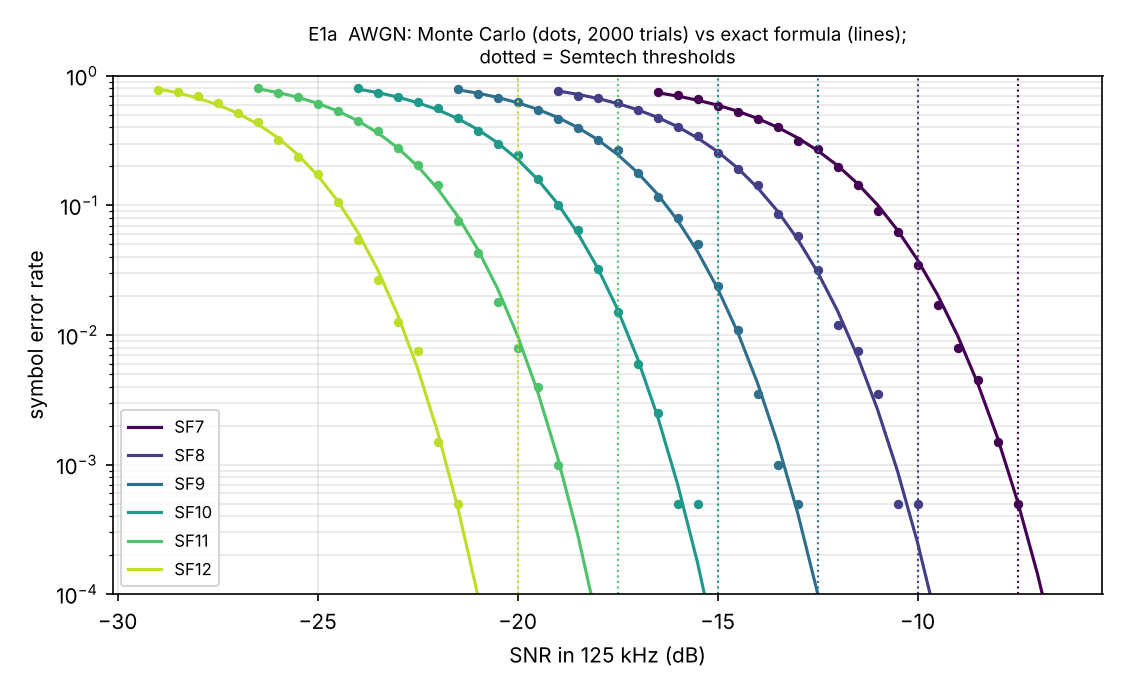
\includegraphics[width=\columnwidth]{../results/e1a_ser_vs_snr_awgn.png}\\[-1mm]
{\small (a)}\\
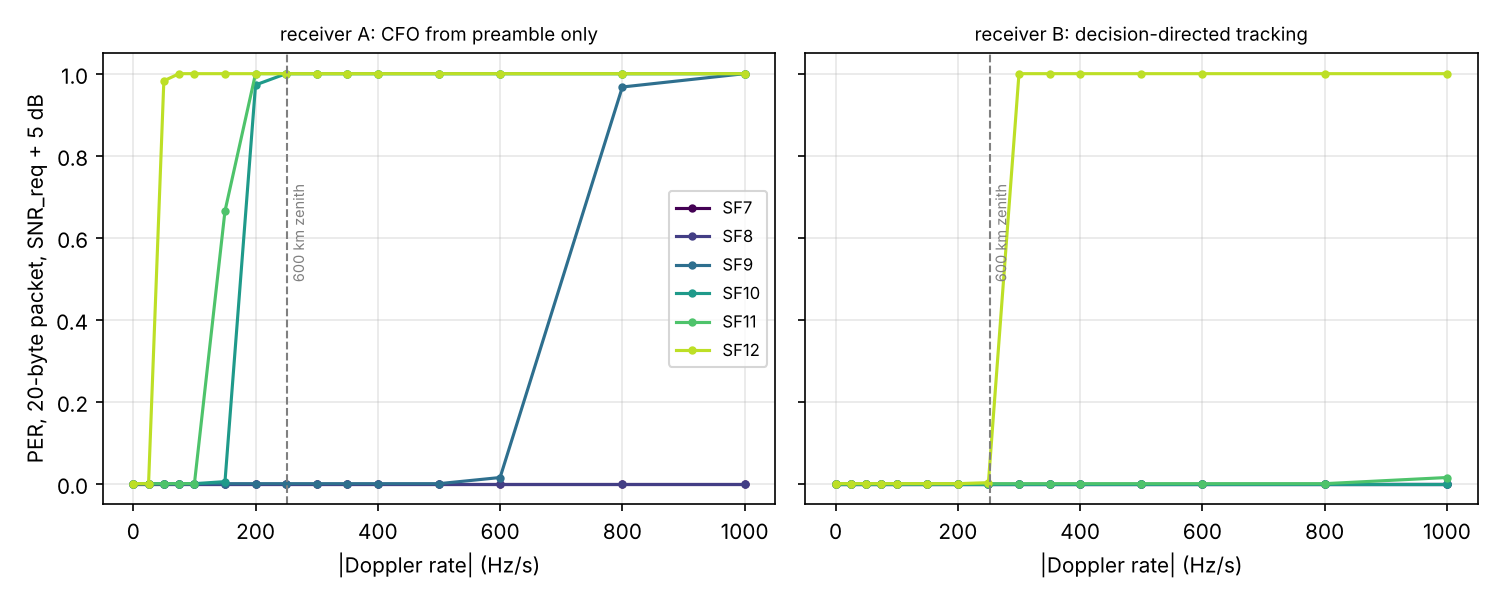
\includegraphics[width=\columnwidth]{../results/e1b_per_vs_doppler.png}\\[-1mm]
{\small (b)}
\caption{E1. (a) SER in AWGN, Monte Carlo (dots) vs exact formula (lines). (b) PER of a 20-byte
packet vs Doppler rate at SNR$_\text{req}$+5\,dB for both receivers.}
\label{fig:e1}
\end{figure}

\subsection{E2 -- Satellite pass}
A 600\,km zenith pass stays above 10$^\circ$ for \EtwoDuration{}\,min, with Doppler up to
$\pm$\EtwoMaxDoppler{}\,kHz, a rate of \EtwoMaxRate{}\,Hz/s at zenith, a one-way delay of
\EtwoDelayMin{}--\EtwoDelayMax{}\,ms and a LOS SNR from \EtwoSnrMin{} to \EtwoSnrMax{}\,dB at 14\,dBm
(Fig.~\ref{fig:e2}). The link only closes at SF$\ge$9 and only near zenith for SF9--10: exactly where the
Doppler rate is highest. With receiver~A, SF12 is usable on \EtwoAshareSFtwelve\,\% of the pass
(\EtwoAshareSFtwelveSnr\,\% if Doppler is ignored): \emph{the most robust SF on the ground is the most
fragile in orbit}, and no single SF is usable over the whole pass: the right SF changes with the
elevation within minutes, far faster than ADR's 20-uplink history. With receiver~B,
SF12 only fails around zenith (usable on \EtwoBshareSFtwelve\,\% of the pass).

The altitude sweep (Fig.~\ref{fig:e2b}) is a check against measurements: with receiver~B, SF12 is
feasible at zenith from \EtwoBSFtwelveZenithFrom\,km upwards (PER $\le$ 1\,\%), while Doroshkin
et al.\ measured SF12 failing near zenith below about 550\,km~\cite{doroshkin2019}, where our zenith
rate is \EtwoRateFiveFifty\,Hz/s. Receiver~B is therefore close to, and slightly more pessimistic than,
real hardware; receiver~A is far too pessimistic. Receiver~B is used in all network experiments.

\begin{figure}[t]
\centering
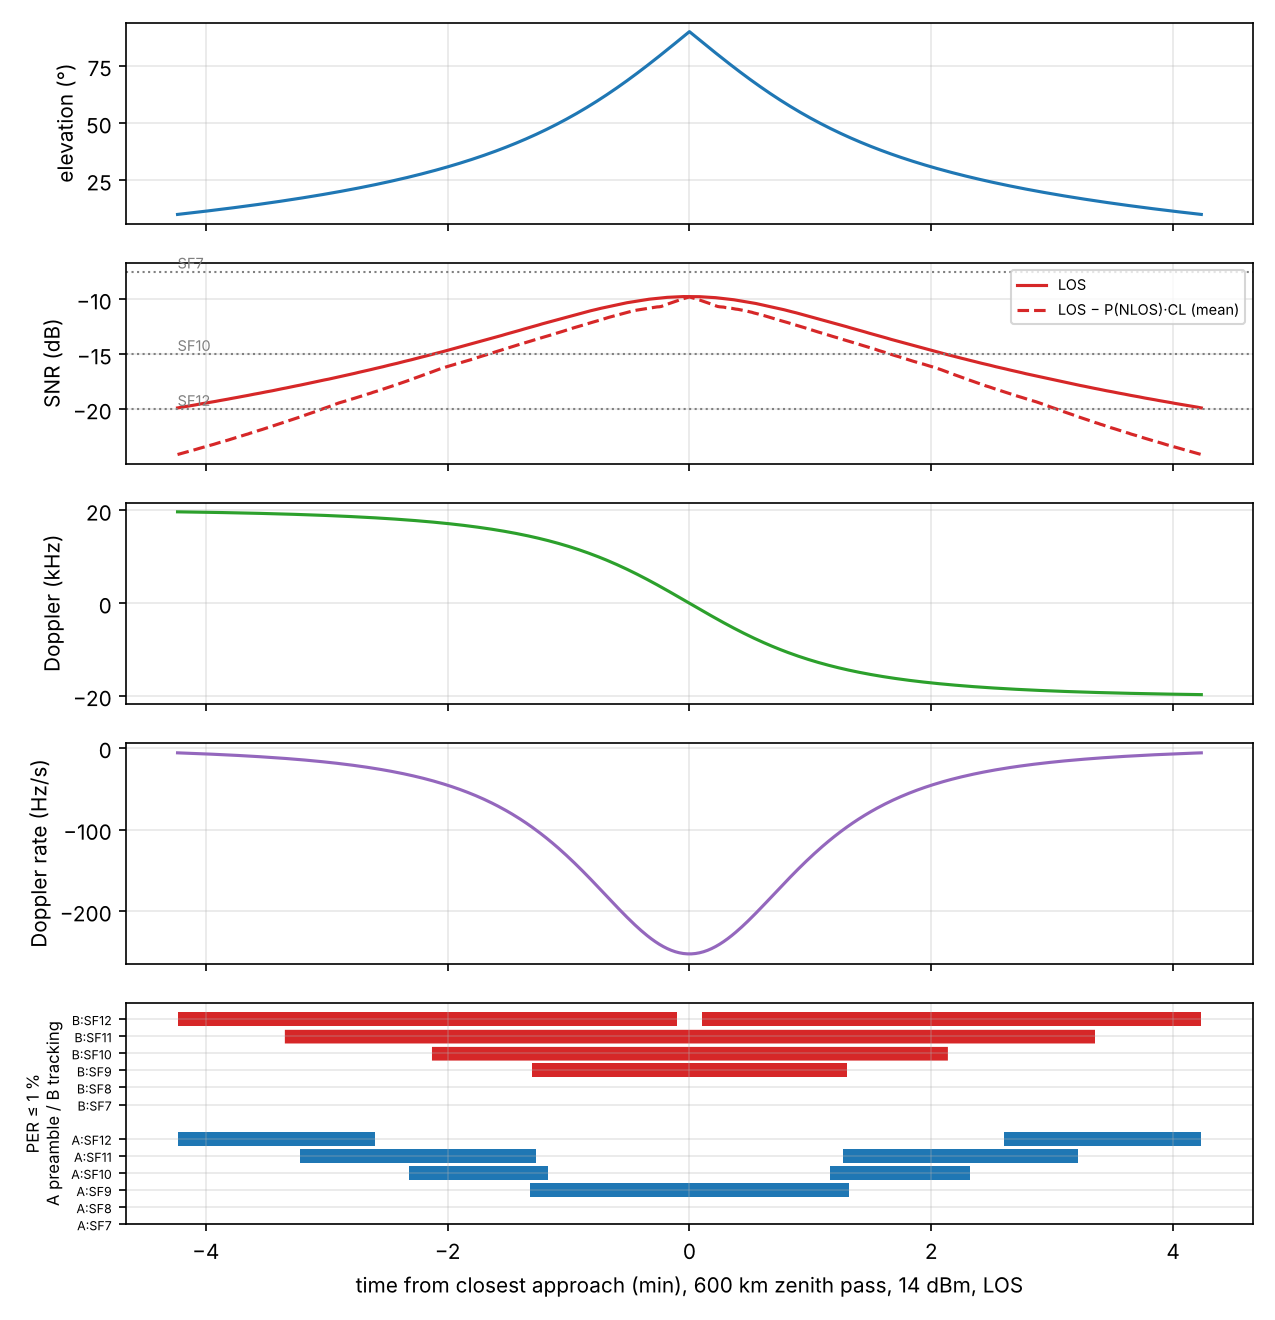
\includegraphics[width=\columnwidth]{../results/e2_satellite_pass.png}
\caption{E2. 600\,km zenith pass: elevation, SNR, Doppler, Doppler rate, and SFs with PER $\le$ 1\,\%
for receivers A and B.}
\label{fig:e2}
\end{figure}

\begin{figure}[t]
\centering
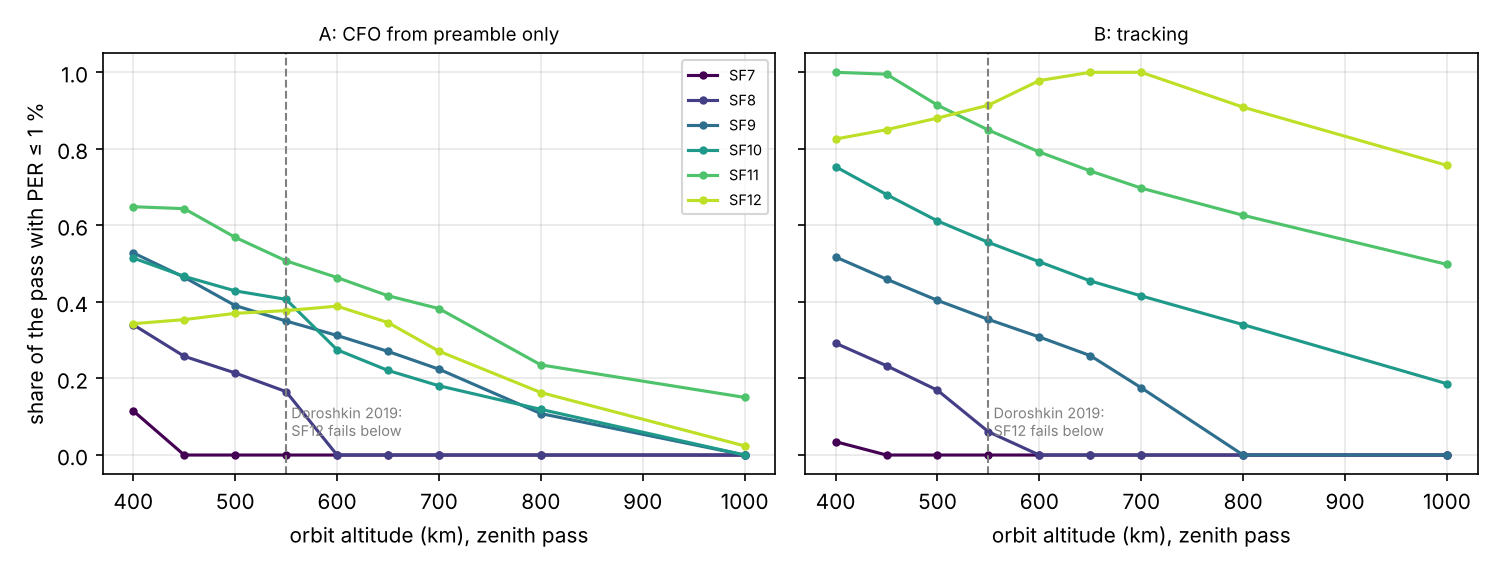
\includegraphics[width=\columnwidth]{../results/e2b_altitude_sweep.png}
\caption{E2b. Share of a zenith pass where each SF reaches PER $\le$ 1\,\%, vs orbit altitude.}
\label{fig:e2b}
\end{figure}

\subsection{E3 -- Scalability without anomalies}
The simulator reproduces pure ALOHA ($|S-Ge^{-2G}|\le$\,\AlohaMaxErr{} up to $G=$\AlohaMaxG{}).
In a terrestrial cell (Fig.~\ref{fig:e3}), ADR delivers \EthreePdrADRLo\,\% of the packets at
$N=\EthreeNlo$ and \EthreePdrADRHi\,\% at $N=\EthreeNhi$, at \EthreeEADRHi\,mJ per delivered packet.
Fixed SF12 collapses with load (\EthreePdrSFtwelveHi\,\% at $N=\EthreeNhi$) because each packet
occupies the channel for 1.3\,s; fixed SF7 stays near \EthreePdrSFsevenHi\,\% because distant devices
cannot reach the gateway. The oracle wins at low load (\EthreePdrOracleLo\,\%) but loses to ADR at
$N=\EthreeNhi$ (\EthreePdrOracleHi\,\%): choosing the lowest energy per packet puts most devices on
SF7 and increases same-SF collisions, while ADR's 10\,dB margin spreads devices over SFs.
The classifier trained on oracle labels under-provisions (\EthreePdrMLHi\,\% at $N=\EthreeNhi$): it
imitates an oracle that knows each packet's fading, and the most likely label given the observable
features is a too-low power or SF. Triggered-Rules is identical to ADR here (no event, no action),
which checks that the triggers stay quiet in normal conditions. The LLM agent equals ADR up to
$N=\EthreeAgentEqualUpTo$ but is below it in \EthreeAgentLossRuns{} of its \EthreeAgentRuns{} runs at
higher load (worst seed \EthreeAgentWorst{} points at $N=\EthreeAgentWorstN$): each time, a false
detector alert coincided with a periodic review and the model moved every device to SF12.

\begin{figure*}[t]
\centering
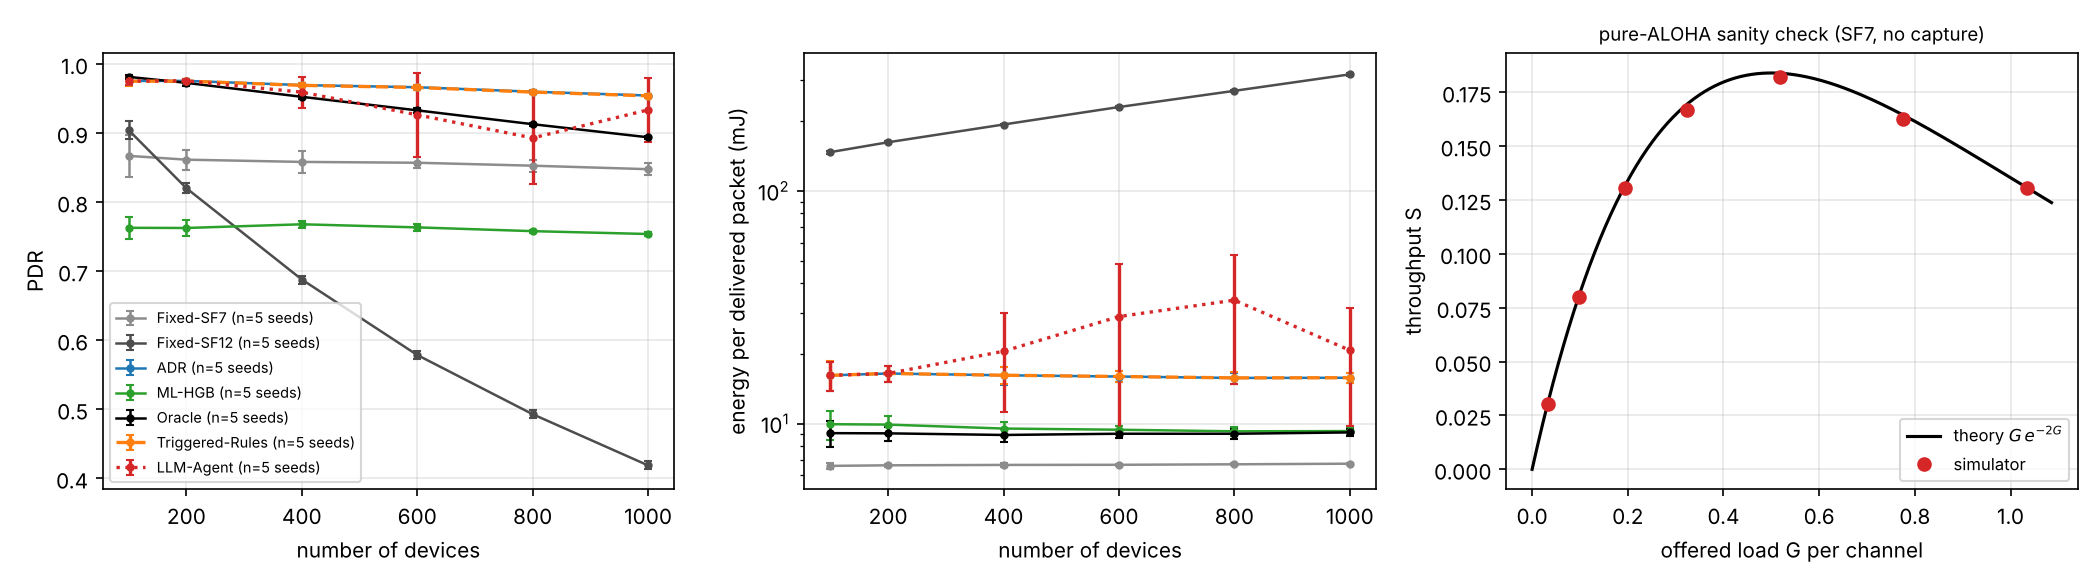
\includegraphics[width=0.95\textwidth]{../results/e3_scalability.png}
\caption{E3. PDR and energy per delivered packet vs number of devices (mean $\pm$ std, 5 seeds), and
the pure-ALOHA check.}
\label{fig:e3}
\end{figure*}

\subsection{E4 -- Anomaly scenarios}
\begin{figure*}[t]
\centering
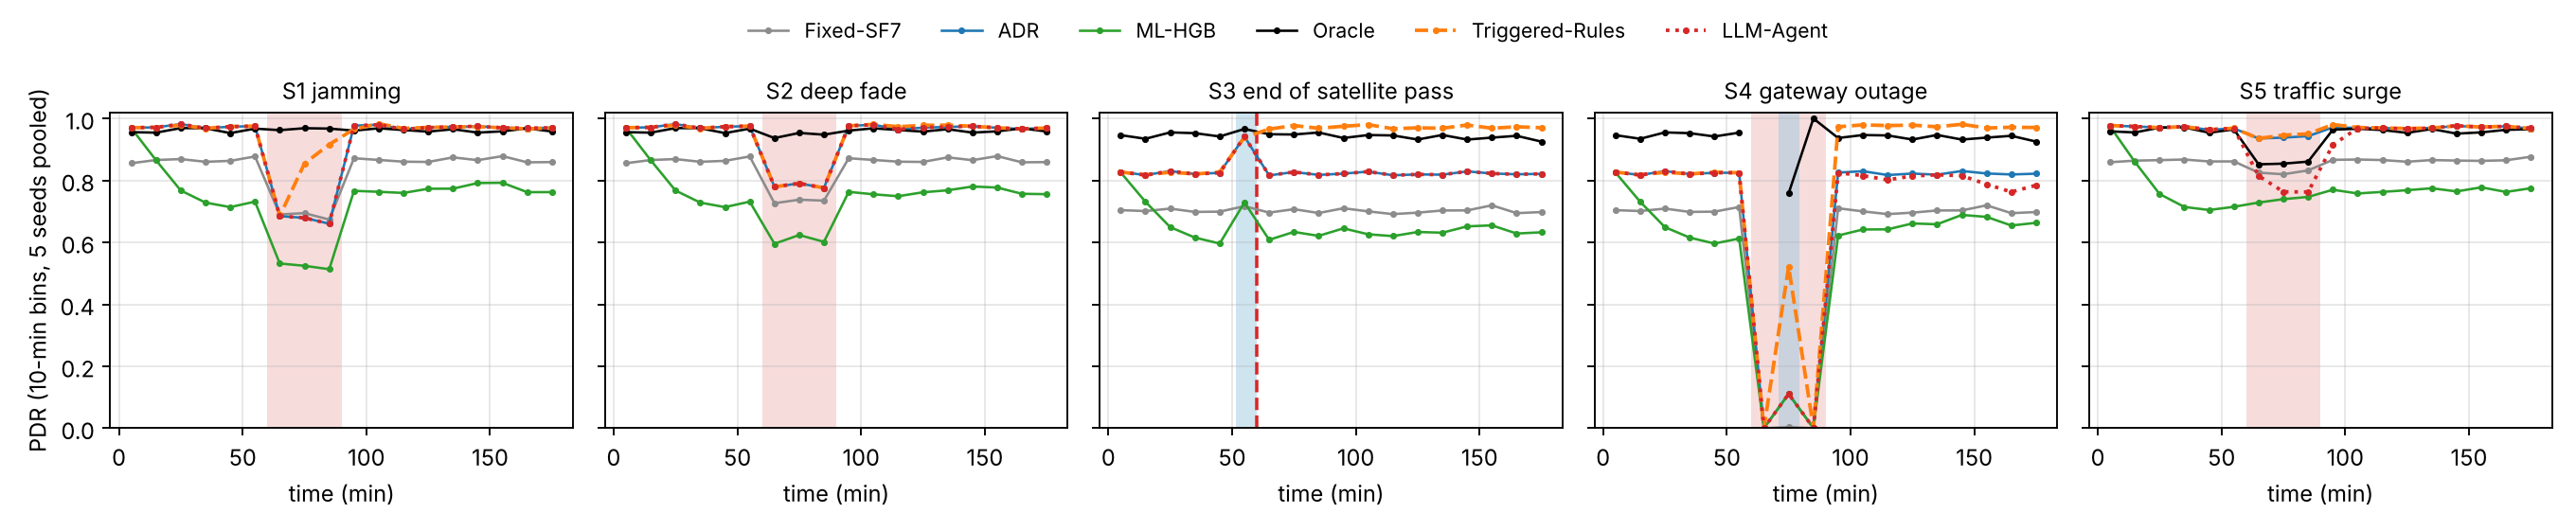
\includegraphics[width=\textwidth]{../results/e4_pdr_timeline_wide.png}
\caption{E4. PDR over time around the five events (10-min bins pooled over 5 seeds; red: event,
blue: satellite pass). Fixed SF12 is off-scale and omitted. LLM agent: Qwen3-0.6B.}
\label{fig:e4}
\end{figure*}
\begin{figure}[t]
\centering
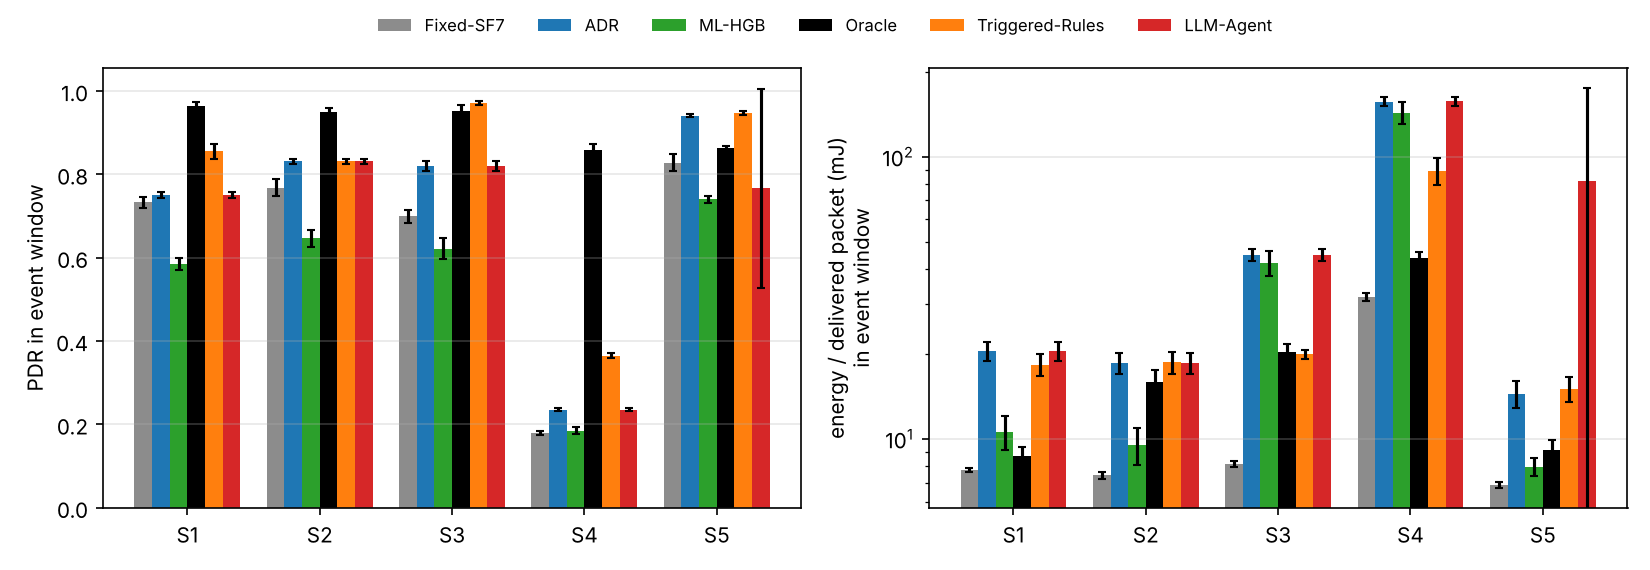
\includegraphics[width=\columnwidth]{../results/e4_event_bars.png}
\caption{E4. Event-window PDR and energy per delivered packet (mean $\pm$ std, 5 seeds).}
\label{fig:e4bars}
\end{figure}
Fig.~\ref{fig:e4} shows the PDR over time and Table~\ref{tab:e4} the event-window PDR with the
paired difference to ADR (same seeds, same channel realisations).

\emph{ADR} keeps the network healthy in normal conditions but does not react to events within
their duration: during jamming its PDR falls to \SOnePdrADR\,\% in the event window and only
recovers when the jammer stops (\SOneRecADR\,min), because ADR can only raise power, never the SF, and
decides on 20-uplink histories.

\emph{Triggered-Rules} --- the same triggers, information and lease mechanism as the agent, with
hand-written rules --- improves the event-window PDR by \SOneDiffRules{} points under jamming,
\SThreeDiffRules{} at the end of the pass and \SFourDiffRules{} during the gateway outage, on every
seed, and halves the energy per delivered packet in S3 (\SThreeERules{} vs \SThreeEADR\,mJ). The
event-triggered architecture is therefore worth about ten points by itself; this is the bar an LLM
agent has to clear. No network-side controller helps against the deep fade (S2,
\STwoDiffRules{} points): under class~A a command needs a delivered uplink, and faded devices are
silent. Only the oracle, which acts instantly and sees the fade, recovers (\STwoDiffOracle{} points).

The \emph{oracle} is the upper bound in S1--S4 but ends \SFiveDiffOracle{} points relative to ADR in
the traffic surge: it minimises the energy of each packet in isolation, which puts most devices on SF7
and multiplies same-SF collisions. The \emph{ML classifier} trained on its labels inherits this
myopia and adds under-provisioning (\SOneDiffML{} points in S1).

\emph{The LLM agent} (Qwen3-0.6B~\cite{qwen3}, \AgentRuns{} runs, \AgentDecisions{} decisions) read the network
correctly with the tools but applied a change only \AgentAppliedTotal{} times; over E3 and E4,
\AgentAppliedTemplate{} of its \AgentAppliedAll{} applied changes were the same action, every device
to SF12 at 10\,dBm. It is identical to
ADR in S1--S3 (\SOneDiffAgent, \STwoDiffAgent{} and \SThreeDiffAgent{} points). In S5 its
event-window PDR was \SFiveDiffAgent{} $\pm$ \SFiveDiffSdAgent{} points relative to ADR, with a loss on
\SFiveLossesAgent{} of 5 seeds: at the
onset of the surge it moved every device to SF12 at 10\,dBm for 30\,min; an SF12 packet occupies
the channel 23 times longer than an SF7 packet, the SF of most devices, while the traffic was five
times higher. In one of the two runs its final message even stated that no change was required. The
action was valid (in range, read-before-write respected), so the
schema guardrail accepted it.



\begin{table}[t]
\caption{E4: event-window PDR (\%, mean $\pm$ std over 5 seeds) and paired difference to ADR (points;
seeds better / worse).}
\label{tab:e4}
\centering\scriptsize
\setlength{\tabcolsep}{2.5pt}
\begin{tabular}{@{}lccccc@{}}
\toprule
& S1 jam & S2 fade & S3 pass end & S4 outage & S5 surge\\
\midrule
ADR & \SOnePdrADR$\pm$\SOnePdrSdADR & \STwoPdrADR$\pm$\STwoPdrSdADR & \SThreePdrADR$\pm$\SThreePdrSdADR & \SFourPdrADR$\pm$\SFourPdrSdADR & \SFivePdrADR$\pm$\SFivePdrSdADR\\
Fixed SF7 & \SOnePdrSFseven & \STwoPdrSFseven & \SThreePdrSFseven & \SFourPdrSFseven & \SFivePdrSFseven\\
Fixed SF12 & \SOnePdrSFtwelve & \STwoPdrSFtwelve & \SThreePdrSFtwelve & \SFourPdrSFtwelve & \SFivePdrSFtwelve\\
ML-HGB & \SOnePdrML & \STwoPdrML & \SThreePdrML & \SFourPdrML & \SFivePdrML\\
Trig.-Rules & \SOnePdrRules & \STwoPdrRules & \SThreePdrRules & \SFourPdrRules & \SFivePdrRules\\
\quad $\Delta$ & \SOneDiffRules{} (\SOneWinsRules/\SOneLossesRules) & \STwoDiffRules{} (\STwoWinsRules/\STwoLossesRules) & \SThreeDiffRules{} (\SThreeWinsRules/\SThreeLossesRules) & \SFourDiffRules{} (\SFourWinsRules/\SFourLossesRules) & \SFiveDiffRules{} (\SFiveWinsRules/\SFiveLossesRules)\\
LLM agent & \SOnePdrAgent & \STwoPdrAgent & \SThreePdrAgent & \SFourPdrAgent & \SFivePdrAgent$\pm$\SFivePdrSdAgent\\
\quad $\Delta$ & \SOneDiffAgent{} (\SOneWinsAgent/\SOneLossesAgent) & \STwoDiffAgent{} (\STwoWinsAgent/\STwoLossesAgent) & \SThreeDiffAgent{} (\SThreeWinsAgent/\SThreeLossesAgent) & \SFourDiffAgent{} (\SFourWinsAgent/\SFourLossesAgent) & \SFiveDiffAgent{} (\SFiveWinsAgent/\SFiveLossesAgent)\\
Oracle & \SOnePdrOracle & \STwoPdrOracle & \SThreePdrOracle & \SFourPdrOracle & \SFivePdrOracle\\
\bottomrule
\end{tabular}
\end{table}

The detector, scored on the ADR runs, reaches an alert precision of \DetPrecision{} and a recall of
\DetRecall{}; it flags jamming within \SOneDetDelay\,min and the outage within \SFourDetDelay\,min, but
the deep fade only after \STwoDetDelay\,min, because faded devices fall silent instead of reporting a
lower SNR.

\subsection{E5 -- Cost of the agent}
\begin{figure}[t]
\centering
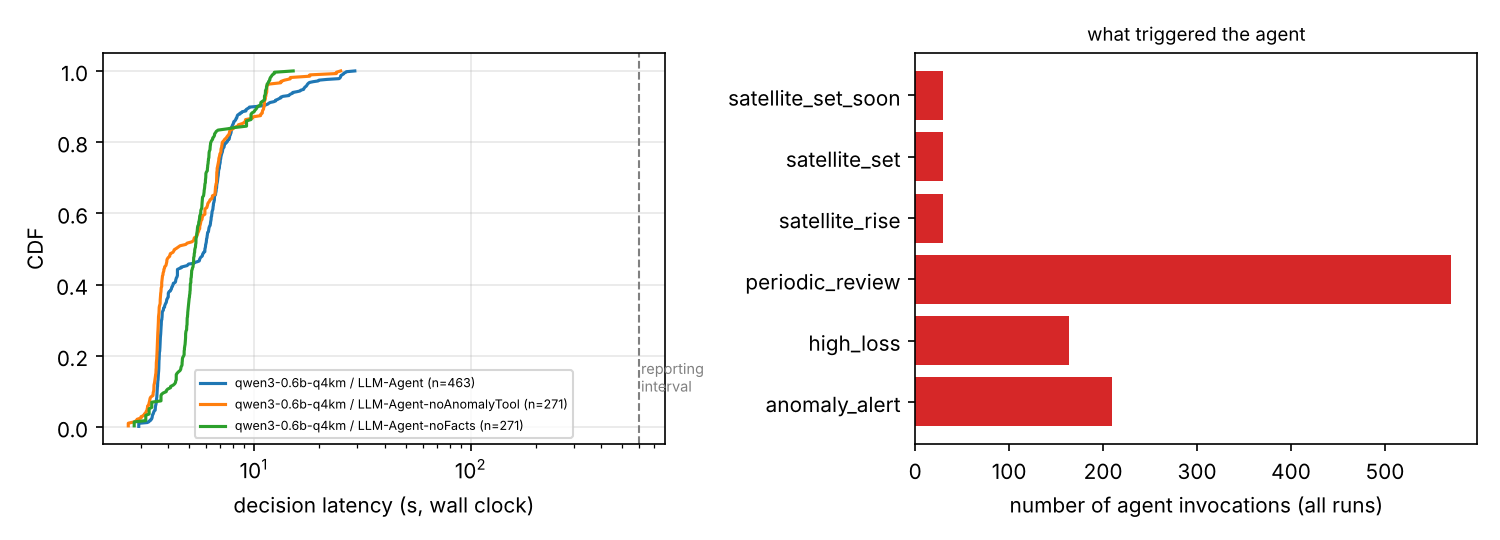
\includegraphics[width=\columnwidth]{../results/e5_agent_cost.png}
\caption{E5. Agent decision latency (CDF, wall clock, 2 CPU threads) and what triggered the agent.}
\label{fig:e5}
\end{figure}
On 2 CPU threads, a decision takes \AgentLatMed\,s (median) and \AgentLatPninetyfive\,s (95th
percentile), with \AgentToolsPerDec{} tool calls and \AgentCallsHour{} LLM calls per simulated hour,
most of them periodic reviews (Fig.~\ref{fig:e5}). This is two orders of magnitude below the 10-min
reporting interval: the reaction delay is set by class-A delivery (up to one reporting period), not
by the model. \AgentSetRejected{} of the \AgentSetCalls{} \texttt{set\_tx\_params} calls were
rejected (invalid-action rate \AgentInvalid\,\%), all for an empty target group; there was no
read-before-write violation (\AgentRbw) and no backend failure.

\subsection{E6 -- Ablations}
Removing the anomaly tool or the LoRa facts from the prompt made the 0.6B model entirely passive:
over \DecisionsNoTool{} and \DecisionsNoFacts{} decisions it applied \AppliedNoTool{} and
\AppliedNoFacts{} changes, read one tool per decision and stopped. Both variants are therefore
identical to ADR in every scenario, including S5 (\SFivePdrNoTool\,\% and \SFivePdrNoFacts\,\% against
\SFivePdrAgent\,\% for the full agent, Fig.~\ref{fig:e6}). For this model, the context that makes it
act is also what makes it harmful; an ablation can only show the value of a component if the full
agent has some, which a larger model may provide.

\begin{figure}[t]
\centering
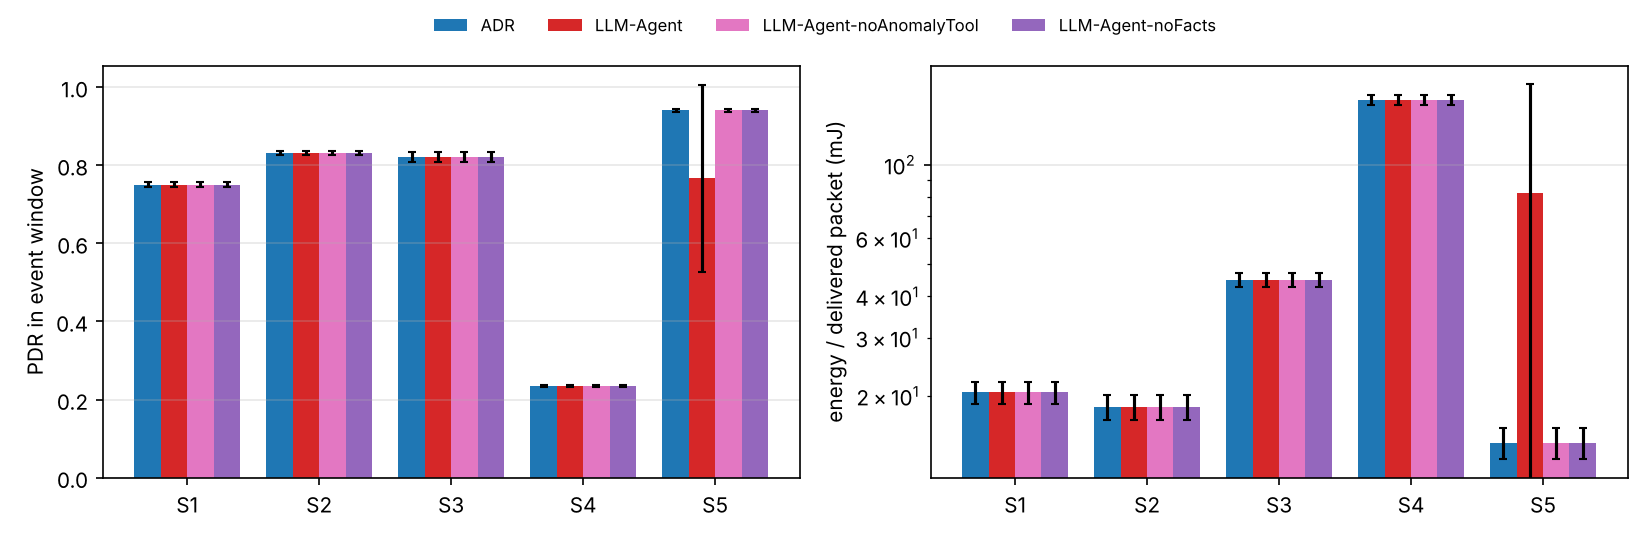
\includegraphics[width=\columnwidth]{../results/e6_ablations.png}
\caption{E6. Event-window PDR and energy per delivered packet for ADR, the full agent and the two
ablations (Qwen3-0.6B, 5 seeds).}
\label{fig:e6}
\end{figure}


\FloatBarrier
\section{Discussion}
\label{sec:discussion}

\textbf{Answer to the research question.} With a 0.6B model, no: the agent did not beat ADR in any
scenario, degraded the network in the traffic surge and under heavy load, and its few actions were
almost always the same template rather than a response to the observed event. The event-triggered architecture, however,
is clearly useful: the same triggers, telemetry and leased overrides driven by six hand-written
rules gain 10--15 points in three of the five scenarios. An LLM agent is only worth its cost if it
beats that rule set, for instance on combinations of events that no rule anticipates. Whether a
3B--7B model clears that bar is the next measurement; the scripts run unchanged with Ollama
(\texttt{--backend ollama --model qwen2.5:3b}).

\textbf{Validated is not safe.} Range validation, the read-before-write rule and the tool cap all
held, yet the agent's only recurrent action (every device to SF12) was harmful during a surge, and in
one run its explanation contradicted its action. We tested a predicted-load check (reject an action whose
offered load would exceed the ALOHA optimum $G=0.5$) and found that it would not have blocked this
case, because the surge had not been observed yet when the agent acted. Effective protection needs
to act on consequences: roll an override back when the measured loss rises after it, apply it first
to a subset of devices, or simulate it in a digital twin of the network before applying it --- the
simulator of this work could serve as that twin.

\textbf{Physics first.} The Doppler rate makes the best SF over a LEO pass change within minutes,
much faster than ADR's 20-uplink history, and whether SF12 survives near zenith depends on the
receiver's frequency tracking (Fig.~\ref{fig:e2b}). A controller that knows the ephemeris and the
receiver's Doppler limits can choose the SF from the elevation; ADR cannot.

\textbf{The control plane bounds every controller.} Under class~A, a command waits for the next
delivered uplink. Agent latency (seconds) is negligible against this delay (minutes), and a deep
fade cannot be fixed from the network at all; only device-side logic or class~B/C downlinks could.

\textbf{Oracles and imitation.} A per-packet oracle that minimises energy is not an upper bound under
heavy load, and a classifier that imitates it without its information under-provisions. Labels
should target an expected PER given what the network can observe, and should account for collisions.

\textbf{Limitations.} No Earth rotation; S-band TR~38.811 tables at 868\,MHz; orthogonal SFs; no
background traffic at the satellite; a broadcast satellite downlink is assumed; one pass per
scenario and 3\,h horizons; receivers A and B are models, not the Semtech demodulator; the agent
results come from a 0.6B model run through llama.cpp because the development environment could not
reach Ollama. All assumptions are listed in the repository (\texttt{docs/ASSUMPTIONS.md}).

\section{Conclusion}
We built a reproducible, Doppler-aware simulation of a hybrid terrestrial--LEO LoRa network and
evaluated an event-triggered LLM agent against fixed SFs, ADR, an ML classifier, an oracle and a
rule-based controller on the same triggers. The physical layer reproduces the measured SF12 limit
of LEO links within about 100\,km of altitude. The event-triggered architecture gains about ten
points of delivery ratio during jamming, satellite pass ends and gateway outages. A 0.6B agent did
not exploit it and once caused harm that schema validation could not stop. Next steps: the 3B and
7B models, a consequence-aware safety layer, store-and-forward buffering, and several passes per
day with Earth rotation.


\IfFileExists{IEEEtran.bst}{\bibliographystyle{IEEEtran}}{\bibliographystyle{ieeetr}}
\bibliography{refs}

\end{document}
